\section{Current Progress}
\label{sec:current_progress}

Substantial progress has been achieved across theoretical design, empirical evaluation, benchmark curation, and system deployment:

\begin{itemize}[leftmargin=*]
    \item \textbf{Academic Publications \& Milestones:} An initial paper detailing the dual-stream morphological gated fusion model and contrastive learning baseline has been accepted for oral presentation at \textbf{AIST 2026} and will appear in Springer LNCS. A full-length manuscript detailing the Kazakh-FEVER 3K benchmark, Hard NEI protocol, and continuous Trust Matrix has been submitted to the \textbf{COLING 2027 ARR track}.
    \item \textbf{Dataset Construction (Kazakh-FEVER 3K):} We curated the first human-validated fact verification benchmark for Kazakh, comprising 3,000 balanced claims across 8 domains (history, geography, science, politics, society, culture, sports, economics: 1,000 \textsc{Supports}, 1,000 \textsc{Refutes}, 1,000 \textsc{NEI}), including 500 Hard NEI counterfactuals, with 100\% agreement on gold controls ($\kappa = 0.84$).
    \item \textbf{Algorithmic Implementation \& Empirical Validation:} The dual-stream model achieves an ROC-AUC of \textbf{0.9980 (Macro)} and F1 of 0.9842 on the Tri-Domain benchmark, outperforming fine-tuned mBERT, XLM-RoBERTa, and zero-shot LLMs. Under out-of-domain evaluation on the Kaspi customer review benchmark, it achieves a \textbf{+42.18 percentage point gain} over vanilla transformers with inference latency $< 85\text{ ms}$ per chunk. Document-level chunking achieves \textbf{100.0\% tamper localization precision}. Figure~\ref{fig:trust_matrix_validation} demonstrates empirical sample separation across the four trust quadrants.
    \item \textbf{Engineering Prototype \& Cloud Deployment:} We engineered a production-grade 4-tab interactive Gradio laboratory deployed to Hugging Face Spaces, featuring: (1) document attribution heatmaps up to 25,000 words, (2) live FST morpheme decomposition, (3) Kazakh-FEVER retrieval and cross-encoder workbench, and (4) interactive 2D Trust Matrix radar.
\end{itemize}

\begin{figure}[htbp]
\centering
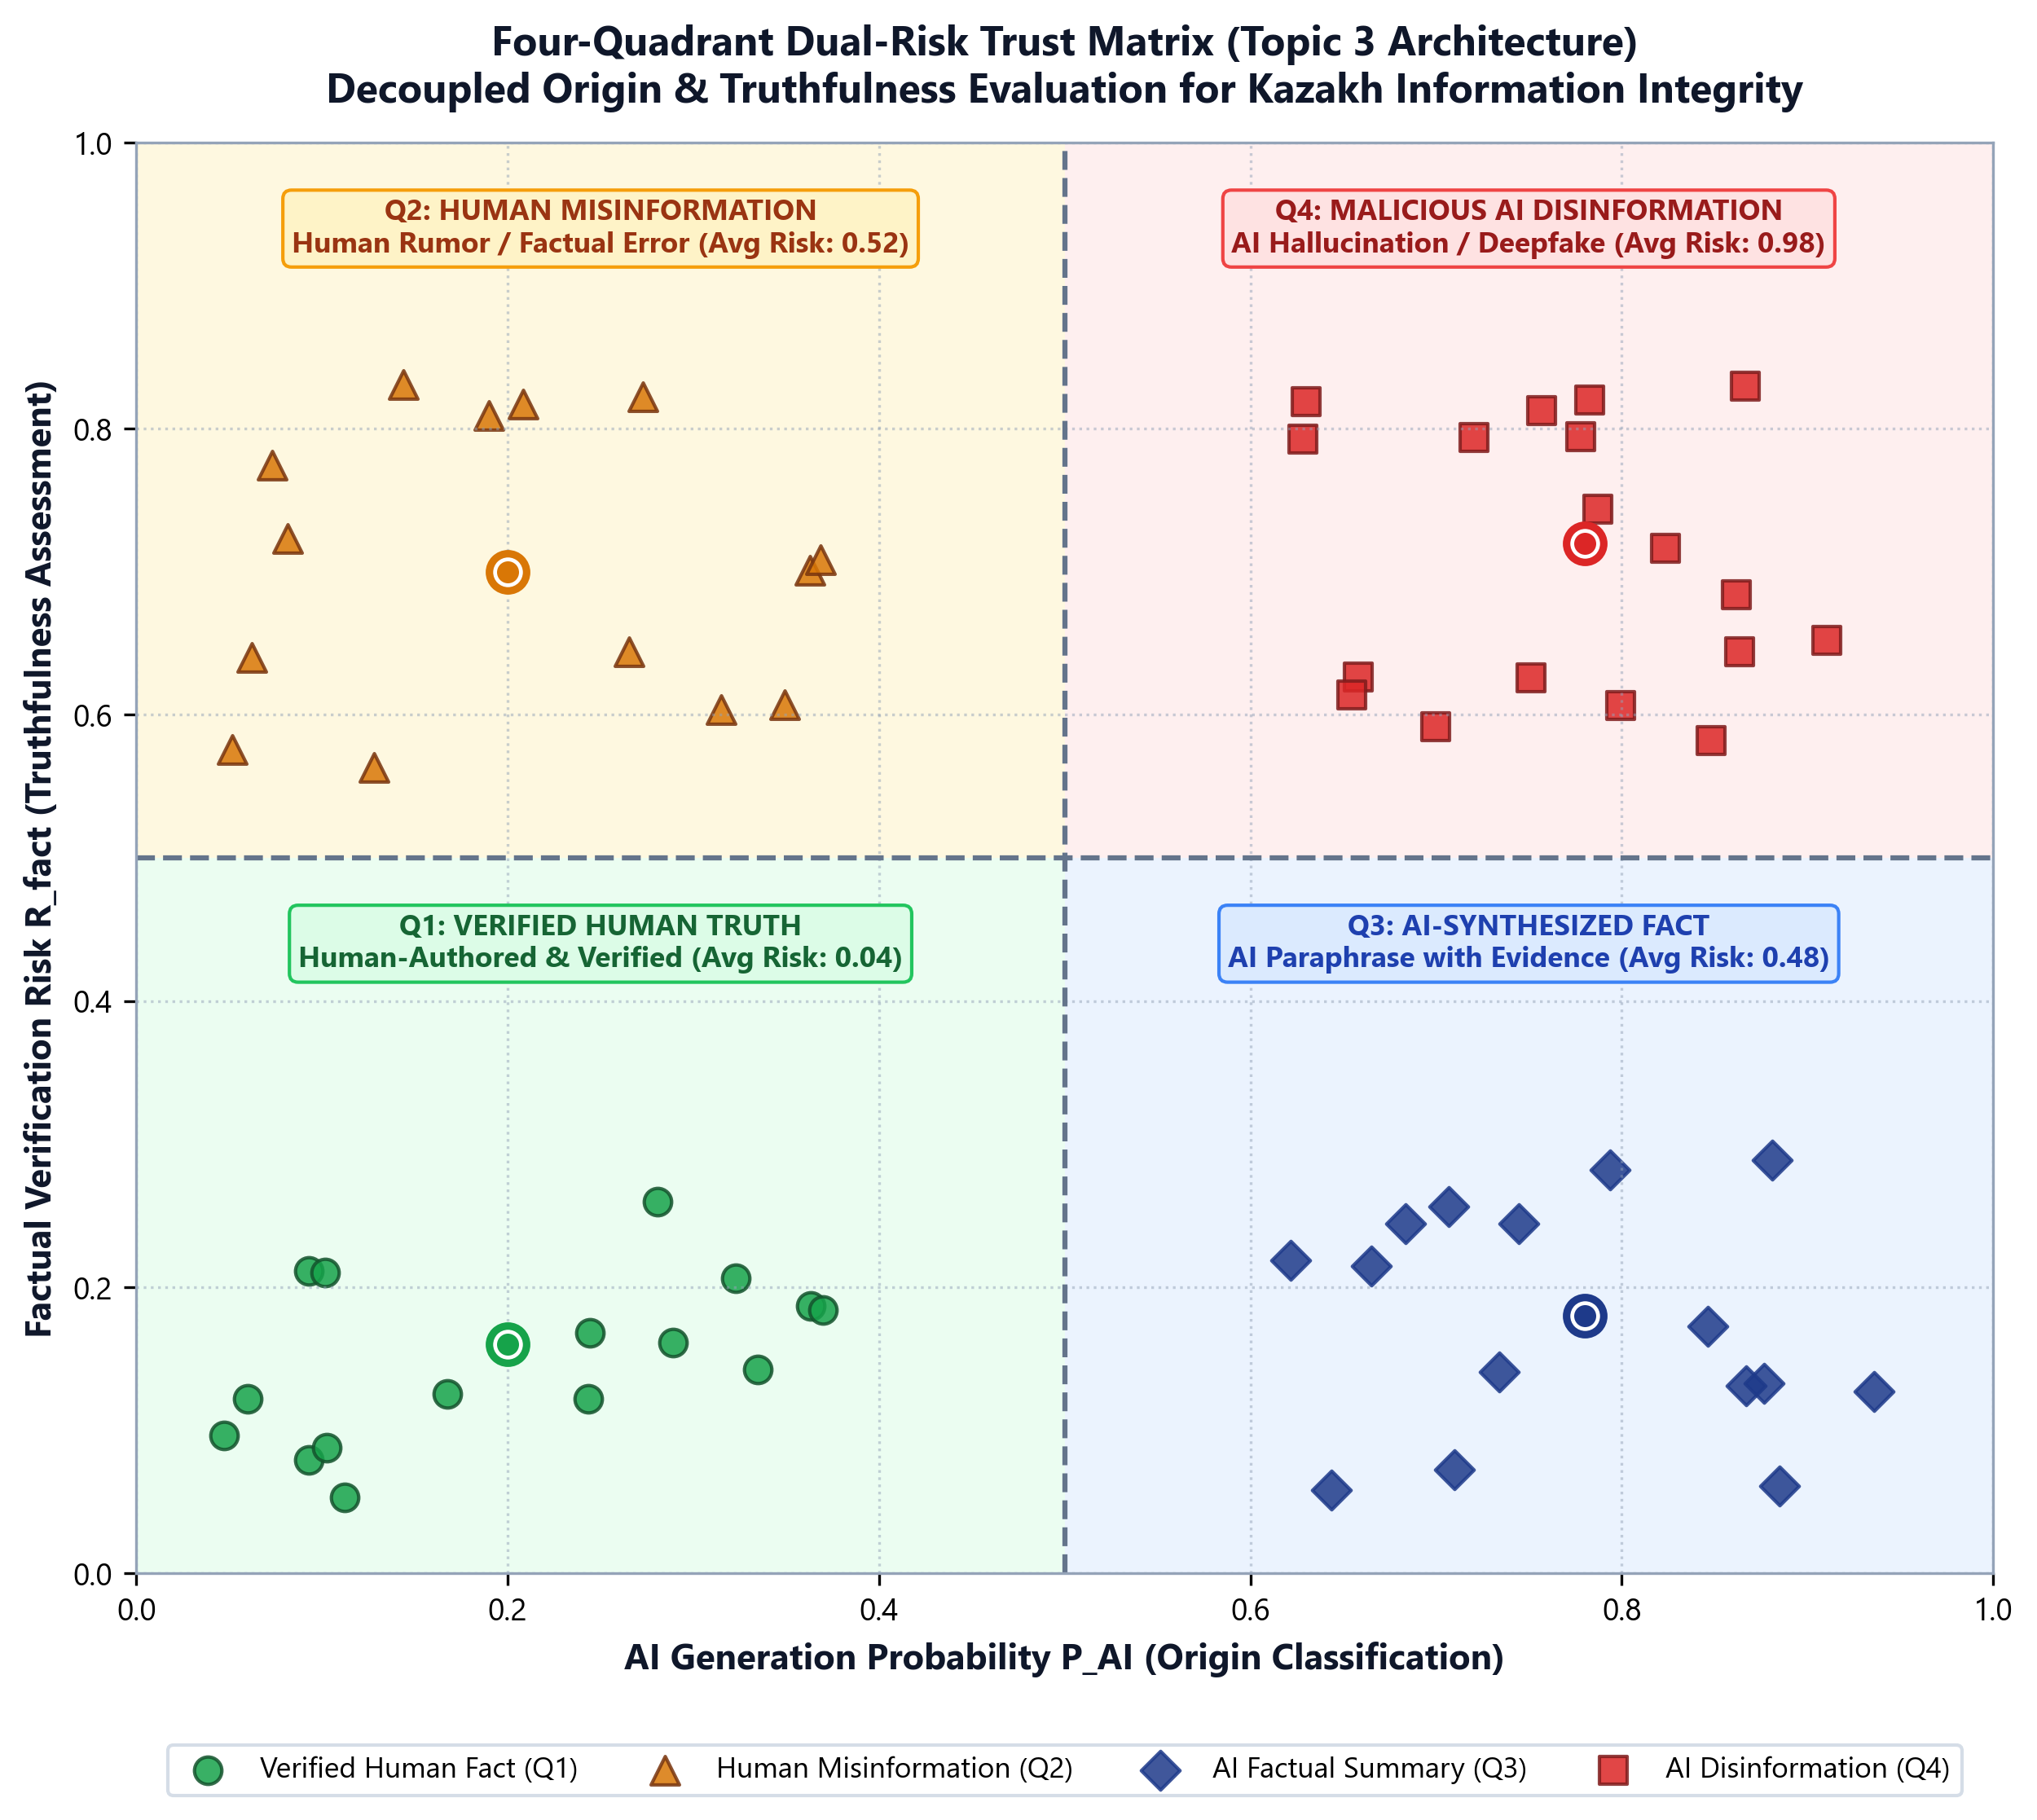
\includegraphics[width=0.72\textwidth]{figures/fig6_trust_matrix_validation.png}
\caption{Four-Quadrant Dual-Risk Trust Matrix Empirical Validation and Decision Boundaries.}
\label{fig:trust_matrix_validation}
\end{figure}
